\documentclass[dvipdfmx,titlepage,a4j]{jsarticle}

\usepackage[top=20mm,bottom=20mm,left=20mm,right=20mm]{geometry}


\usepackage{url}
\usepackage{graphicx}
\usepackage{listings,jvlisting}
\usepackage{amsmath,amssymb}
\usepackage{graphicx}
\usepackage[yen]{okuverb}
\usepackage{ascmac}
\usepackage{fancybox}
\usepackage{fancyvrb}
\usepackage{fancyhdr}
\usepackage{lastpage}
\usepackage{caption}
\usepackage{subcaption}
\usepackage{here}
\usepackage{titling}

% ヘッダーとフッターの設定
\renewcommand{\headrulewidth}{0.2pt} % ヘッダーの線
\renewcommand{\footrulewidth}{0.4pt} % フッターの線

% ヘッダー 
\fancyhead[L]{}
\fancyhead[C]{\thetitle}
\fancyhead[R]{}

% フッター
\fancyfoot[L]{}
\fancyfoot[C]{\thepage / \pageref{LastPage}} % ページ番号
\fancyfoot[R]{}

% lstlistingの設定
\lstset{
  language={C++},
  basicstyle={\ttfamily},
  identifierstyle={\small},
  commentstyle={\smallitshape},
  keywordstyle={\small\bfseries},
  ndkeywordstyle={\small},
  stringstyle={\small\ttfamily},
  frame={tb},
  tabsize={2},
  breaklines=true,
  columns=[l]{fullflexible},
  numbers=left,
  xrightmargin=0zw,
  xleftmargin=3zw,
  numberstyle={\scriptsize},
  stepnumber=1,
  numbersep=1zw,
  lineskip=-0.5ex
}

\author{waarrk}
\date{2023年2月1日}

\begin{document}

\begin{titlepage}
    \centering
    \vspace*{2cm}

    \vspace{5cm}

    {\LARGE \textbf{小惑星表面探査のための\\CubeSat放出型・多脚式自律移動ロボット研究}}

    \vspace{0.5cm}

    {\textbf{千葉工業大学 先進工学部 未来ロボティクス学科}\\}
    {\textbf{22C1704 鷲尾 優作}}

    \vfill

    {\large 2025年5月7日}

    \vspace{1cm}
\end{titlepage}

\newpage

\section{目的}
本計画書は、修士課程の研究計画を明確化し、指導教員との合意形成を図ることを目的とする。

\section{研究背景}
近年、小惑星探査は、地球衝突天体への対処(いわゆるプラネタリーディフェンス)や、
宇宙資源の活用を目的とした探査の観点から、注目を集めている。

従来の小惑星探査機は、サンプル採取ミッションを除けば、探査機本体のリスク低減のため、小惑星表面への極端な接近を避け、
主に上空からのリモートセンシングによって観測を行ってきた。しかし、この方法では表面の微細構造解析に限界がある。
この課題に対処するため、日本の「はやぶさ2」では、表面観測用ロボットの投下が実施され、MINERVA-II1A/B\cite{minelva:online}およびMASCOT\cite{Krause2022}が成果を挙げた(図\ref{fig:hayabusa2})。


\begin{figure}[H]
    \centering
    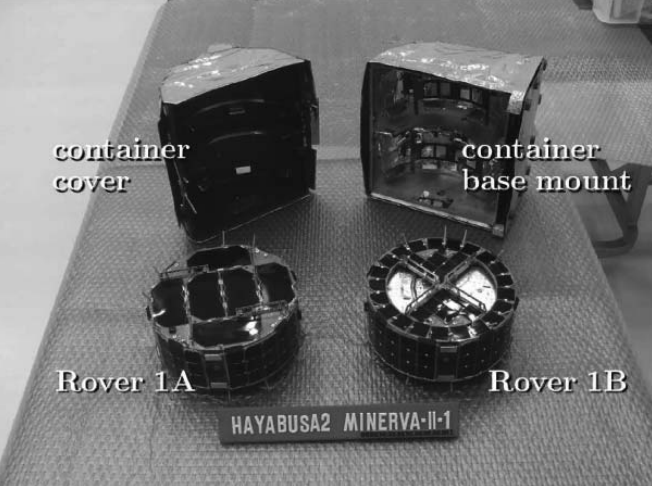
\includegraphics[width=0.5\textwidth]{picture/mine.png}
    \caption{「はやぶさ2」に搭載されたロボット「MINERVA-II-1」}
    \label{fig:hayabusa2}
\end{figure}

MINERVAシリーズはホッピング機構による移動方式を確立したが、任意の地点への精密移動は困難であり、実証用の専用設計のため汎用性には欠けている。
そもそも小惑星表面探査機は、表面の所望する任意の地点に着地しデータを取得できることが理想であるが、
微小重力環境や不整地での運用が求められるため、移動以前に着地の成功そのものが困難である。
初代はやぶさのMINERVA\cite{探査ロボット「ミ5:online}が放出後の方向不良で失敗した事例や、
欧州の彗星探査機ロゼッタ搭載のフィラエ\cite{ESARoset23:online}がアンカー作動不良により意図しない場所に着地した事例など、
着地後の位置制御・固定に課題が存在する。

こうした課題に対し、以下の2つの方向性が考えられる
\begin{itemize}
    \item 探査機の台数を増やし、着地の不確実性を緩和する手法
    \item 各探査機に移動機能を持たせ、着地後に自律的に目的地へ移動する手法
\end{itemize}

後者の点ではETH Zurich大学がSpace Hopperと呼ばれる小惑星向け多脚式ホッピング型ロボットを開発中であり、
脚を用いることで小惑星表面の不整地を移動することが可能となる可能性が示唆されている\cite{SpaceHop55:online}。

\begin{figure}[H]
    \centering
    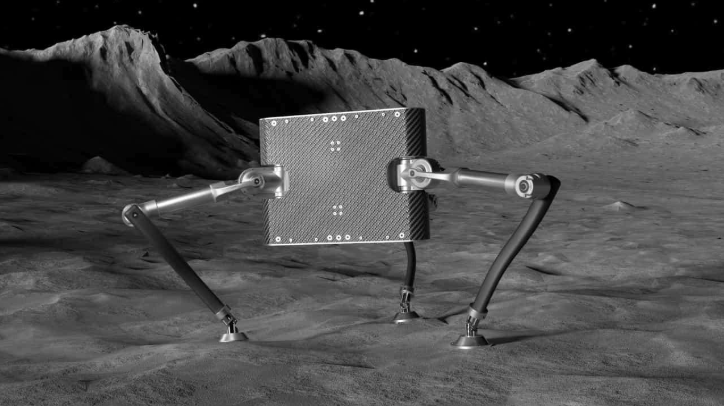
\includegraphics[width=0.5\textwidth]{picture/hopper.png}
    \caption{Space Hopper}
    \label{fig:hopper}
\end{figure}

一方で、近年普及が進むCubeSatは、1U(10cm立方)を基本単位とする規格化された小型衛星であり、低コスト・短期開発を実現している。
ESAの「Hera」ミッションでは2機のCubeSatが深宇宙へ投入され、こうした超小型衛星の応用範囲が拡大しつつある\cite{ESAHeraa1:online}。
また、民間による小惑星探査の試みも活発化しており、マクサー社の「サイキ」や、2028年打ち上げ予定のExLabs社「SERV」に搭載される千葉工業大学製探査機(非移動型)など、
ロボットの小惑星への輸送機会も増加しており、今後、ペイロードはCubeSat放出機構に収容可能なものが主流となると考えられる。
共通の搭載機構を採用すれば、搭載台数も増やしやすいため、着地の不確実性を緩和する手法としても有効である。

以上の背景を踏まえると、CubeSatサイズに準拠した多脚式の移動ロボットを開発することで、これまでの小惑星表面探査における課題の克服が期待できると考えられる。
加えて、共通設計の採用によるコスト削減や、既存の放出機構の流用による開発期間の短縮も見込まれる。

\section{研究目的}
CubeSat放出機構から放出可能な多脚式自律移動ロボットを開発し、
小惑星表面における多点観測を実現可能とする移動探査技術の確立を目指す。

\section{研究内容}
本研究では、以下の2点を中心に取り組む。

\begin{enumerate}
    \item \textbf{機体設計:}
          CubeSat放出機構に収容可能な多脚型機構を設計する。
    \item \textbf{自律制御系:}
          ロボットの搭載コンピュータ上に経路計画アルゴリズムを実装し、任意の観測地点への経路計画を目指す。
\end{enumerate}

設計・開発は、筆者が2025年度に実施する小惑星アポフィス向け探査機の設計知見を踏まえ、後継機としての要求仕様を随時反映しつつ進める。


\section{研究スケジュール}
2025年4月から学部4年時に先行機の設計を行い、2026年4月から修士課程に進学後、移動型ロボット試作機の構想設計を行う。
修士課程入学後は、宇宙科学技術連合講演会、IROS、アストロダイナミクスシンポジウム等の学会において、研究成果を発表する。

\begin{table}[H]
    \centering
    \caption{スケジュール案}
    \begin{tabular}{l|l}
        \hline
        期間           & 内容           \\
        \hline \hline
        2025年4月から12月 & 先行機の開発       \\
        \hline
        2026年1月から3月  & 具体的な後継機の仕様検討 \\
        \hline
        2026年4月頃から   & 試作機構造設計      \\
        \hline
        2027年4月頃から   & 試作機ソフトウェア設計  \\
        \hline
        2027年頃       & 国際学会への論文投稿   \\
        \hline
    \end{tabular}
    \label{tab:schedule}
\end{table}

\section{期待される成果}
CubeSat放出機構と組み合わせて運用可能な自律移動ロボットの試作機が完成する見込みである。小惑星表面探査機において、探査機の冗長性確保や、多点観測の柔軟性向上といった新しい観測手法の確立が期待される。

\newpage

\nocite{*}
\bibliographystyle{jplain}
\bibliography{refs}

\end{document}
